%%
%% This is file `swuthesis-main.tex',
%% generated with the docstrip utility.
%%
%% The original source files were:
%%
%% swuthesis.dtx  (with options: `example')
%% This is a generated file.
%% 
%% It was extracted from swuthesis.dtx.


\begin{filecontents*}[overwrite]{swuthesis-main.bib}
@standard{gbt7714,
  title        = {信息与文献 参考文献著录规则},
  organization = {国家市场监督管理总局、
    国家标准化管理委员会},
  number       = {GB/T 7714---2025},
  year         = {2025},
  address      = {北京},
  publisher    = {中国标准出版社}
}

@book{knuth1984texbook,
  author    = {Donald E. Knuth},
  title     = {The {\TeX}book},
  volume    = {A},
  series    = {Computers and Typesetting},
  publisher = {Addison-Wesley},
  year      = {1984},
  address   = {Reading, MA}
}

@book{lamport1994latex,
  author    = {Leslie Lamport},
  title     = {{\LaTeX}: A Document Preparation System},
  edition   = {2},
  publisher = {Addison-Wesley},
  year      = {1994},
  address   = {Reading, MA}
}

@book{mittelbach2004companion,
  author    = {Frank Mittelbach and Michel Goossens and Johannes Braams
    and David Carlisle},
  title     = {The {\LaTeX} Companion},
  edition   = {2},
  publisher = {Addison-Wesley},
  year      = {2004},
  address   = {Boston}
}

@manual{ctex2022,
  title        = {{CTeX} 宏集手册},
  author       = {{CTeX-org}},
  organization = {CTeX-org},
  year         = {2022},
  note         = {CTAN: https://ctan.org/pkg/ctex. 引用日期: 2026-04-18.},
  langid       = {chinese}
}

@book{zhouzhihua2016ml,
  author    = {周志华},
  title     = {机器学习},
  publisher = {清华大学出版社},
  year      = {2016},
  address   = {北京},
  isbn      = {978-7-302-42328-7},
  langid    = {chinese}
}

@article{liguojie2012bigdata,
  author       = {李国杰 and 程学旗},
  title        = {大数据研究: 未来科技及经济社会发展的重大战略领域——
    大数据的研究现状与科学思考},
  journaltitle = {中国科学院院刊},
  year         = {2012},
  volume       = {27},
  number       = {6},
  pages        = {647--657},
  issn         = {1000-3045},
  langid       = {chinese}
}

@article{WalpuskiZhang2021DMJ,
  author       = {Walpuski, Thomas and Zhang, Boyu},
  title        = {On the Compactness Problem for a Family of Generalized
    {Seiberg--Witten} Equations in Dimension 3},
  journaltitle = {Duke Mathematical Journal},
  shortjournal = {Duke Math. J.},
  volume       = {170},
  number       = {17},
  pages        = {3891--3934},
  year         = {2021},
  doi          = {10.1215/00127094-2021-0005},
  note         = {MathSciNet MR4340726},
  langid       = {english}
}

@misc{taubes2020compactness,
  author     = {Taubes, Clifford Henry},
  title      = {{Compactness for $\mathrm{SL}(2;\mathbb{C})$ and 4D anti-self dual
    equations}},
  year       = {2020},
  eprinttype = {arxiv},
  eprint     = {1307.6447},
  langid     = {english}
}

@inproceedings{vaswani2017attention,
  author    = {Vaswani, Ashish and Shazeer, Noam and Parmar, Niki and Uszkoreit, Jakob
    and Jones, Llion and Gomez, Aidan N. and Kaiser, {\L}ukasz and Polosukhin, Illia},
  title     = {Attention Is All You Need},
  booktitle = {Advances in Neural Information Processing Systems 30:
    Proceedings of the 31st Conference on Neural Information Processing Systems},
  year      = {2017},
  pages     = {5998--6008},
  publisher = {Curran Associates, Inc.},
  address   = {Long Beach, CA, USA},
  langid    = {english}
}

@online{swu2021thesisManageNotice,
  author    = {{西南大学}},
  title     = {关于印发《西南大学全日制本科学生毕业论文（设计）工作管理办法》的通知},
  date      = {2021-01-07},
  url       = {https://ceie.swu.edu.cn/info/1125/3918.htm},
  urldate   = {2026-04-18},
  note      = {西校〔2021〕4号},
  langid    = {chinese}
}

@online{swuUndergradThesisSpecWeb,
  author    = {{西南大学}},
  title     = {西南大学本科毕业论文（设计）规范},
  url       = {https://ceie.swu.edu.cn/info/1125/3918.htm},
  urldate   = {2026-04-18},
  note      = {门户亦可能发布 \texttt{.docx} 直链；以当期页面为准。},
  langid    = {chinese}
}

@online{swu2022gradThesisSpecDoc,
  author    = {{西南大学}},
  title     = {西南大学博士硕士学位论文规范},
  date      = {2022-06-28},
  url       = {https://dwyx.swu.edu.cn/info/1083/2038.htm},
  urldate   = {2026-04-18},
  note      = {西南大学博士硕士学位论文规范.doc},
  langid    = {chinese}
}

@misc{bao2024swuthesisLegacy,
  author       = {包小敏},
  title        = {西南大学本科毕业论文 {\LaTeX} 模板（本科毕业论文模板\_新）},
  year         = {2024},
  month        = aug,
  howpublished = {西南大学数学与统计学院本科毕业论文写作模板；含 myTemplate.tex、SWUthesis.sty 等},
  note         = {持续维护至 2024 年；联系信箱 xbao@swu.edu.cn},
  langid       = {chinese}
}
\end{filecontents*}

\documentclass[bachelor,fontset=macnew, punct=banjiao]{swuthesis}

\usepackage{subcaption}
\usepackage{longtable}
\usepackage{siunitx}
\usepackage{tikz}
\usetikzlibrary{arrows.meta,positioning}
\sisetup{detect-all}

\swusetup{
  title         = {西南大学本科毕业论文模板示例文档},
  subtitle      = {基于 \texttt{swuthesis.dtx} 自动生成的主文档},
  title-en      = {An Example Main Document Generated from \texttt{swuthesis.dtx}},
  college       = {数学与统计学院},
  college-en    = {School of Mathematics and Statistics},
  major         = {数学与应用数学},
  author        = {张三},
  author-en     = {San Zhang},
  student-id    = {222026314210000},
  supervisor    = {李四\ 教授},
  defense-date = {2026/6/18}
}

\addbibresource{swuthesis-main.bib}

\begin{document}

\frontmatter
\maketitle
\tableofcontents
\begin{cnabstract}
本文给出一个面向西南大学本科毕业论文（设计）的 \LaTeX{} 模板示例文档，
重点演示封面与摘要生成、章节结构组织、插图与子图排版、三线表与长表格排版、数学公式编号与引用、
定理环境定义以及参考文献著录等常见功能。示例内容同时吸收学校现行本科毕业论文（设计）规范中的
基本要求、编写格式、排版要求和材料装袋顺序，用于说明如何将正式规范转化为可复用的模板结构。
该示例既可作为模板测试文件，也可作为后续扩展博士、硕士与本科统一文档体系的基础。
附录收录《西南大学本科毕业论文（设计）规范》全文，便于对照。
\end{cnabstract}
\begin{cnkeywords}
西南大学；毕业论文模板；\LaTeX；本科论文；排版示例
\end{cnkeywords}
\begin{enabstract}
This document presents an undergraduate thesis example for Southwest University%
based on \LaTeX.%
It demonstrates the generation of the cover page and bilingual abstract,%
chapter organization, figures and aligned subfigures,%
three-line tables and long tables,%
equation numbering and cross-referencing,%
theorem-like environments, and bibliography formatting.%
The example also incorporates the current undergraduate thesis specification%
of the university,%
so that formal writing requirements can be translated%
into a reusable template structure.%
It is intended both as a regression test for the class file%
and as a starting point for a unified%
document system covering undergraduate, master's, and doctoral theses.
\end{enabstract}
\begin{enkeywords}
Southwest University; thesis template; \LaTeX; undergraduate thesis;%
typesetting example
\end{enkeywords}
\makeabstract

\mainmatter
\chapter{模板制作说明}\label{ch:guide}

本章说明本示例文档的用途，以及模板与学校正式规范之间的关系。%
《西南大学本科毕业论文（设计）规范》为统一本科毕业论文（设计）的撰写和编辑格式，%
保证本科毕业论文（设计）的质量，便利信息系统的收集加工、检索利用和交流传播，%
在《西南大学全日制本科学生毕业论文（设计）工作管理办法》（西校〔2021〕4号）基础上制定%
\cite{swu2021thesisManageNotice,swuUndergradThesisSpecWeb}。%
\textbf{该规范的完整条文已收录于附录~\ref{app:swu-undergrad-spec}}，%
写作与提交时请以学校最新发布的文件为准；若规范修订，请相应更新附录文本或改附说明。%
博士、硕士学位论文的撰写与排版另有《西南大学博士硕士学位论文规范》%
\cite{swu2022gradThesisSpecDoc}（页面提供 \texttt{.doc} 文档下载，以学校及学院最新发布为准）。

\section{编译与工具链}\label{sec:compile}
\subsection{引擎与参考文献后端}
\begingroup\sloppy
正文为中文并依赖字体与 \texttt{ctex}，\textbf{须使用 \hologo{XeLaTeX}} 编译。
参考文献使用 \texttt{biblatex}，\textbf{须运行 \hologo{biber}}（随 TeX~Live、MiKTeX 等发行版安装，版本号随发行版更新；与 \texttt{biblatex} 配套的是名为 \hologo{biber} 的程序，在编辑器中配置「参考文献处理器」时选 \hologo{biber} 即可）。
\textbf{不要使用}以 \hologo{pdfLaTeX} 为默认的一键流程（例如 WinEdt 中常见的 PDF\TeX{}ify），否则无法正确排版中文与参考文献。
\par\endgroup

\subsection{Windows（含 WinEdt）}
\begin{itemize}
  \item \textbf{Biber 与 WinEdt}：WinEdt 不单独「支持某个 biber 版本号」，%
  而是调用发行版已安装的 \hologo{biber}（Windows 下可执行文件名为 \texttt{biber.exe}）。%
  在 \texttt{TeX} $\rightarrow$ \texttt{Execution Modes}（或同类菜单）中，将主流程设为 \textbf{\hologo{XeLaTeX}}，%
  并在需要时增加一步 \hologo{biber}，再多次 \hologo{XeLaTeX}，顺序与下文 Makefile 一致即可。
  \item \textbf{避免 PDF\TeX{}ify}：该快捷方式通常绑定 \hologo{pdfLaTeX}，与本模板不兼容。请改用「\hologo{XeLaTeX} + \hologo{biber} + \hologo{XeLaTeX}」或下文 \texttt{latexmk}。
  \item 若已安装 TeX~Live 并将 \texttt{bin} 加入系统 \texttt{PATH}，也可在「命令提示符」或 PowerShell 中进入工程目录，手动执行与 \cref{sec:compile-make} 相同的命令。
\end{itemize}

\subsection{macOS / Linux 与 \texttt{Makefile}}\label{sec:compile-make}
工程根目录的 \path{Makefile} 会依次执行：%
\hologo{XeLaTeX} $\rightarrow$ \hologo{biber} $\rightarrow$ \hologo{XeLaTeX}%
  $\rightarrow$ \hologo{XeLaTeX}%
（与参考文献、交叉引用完全刷新所需次数一致）。%
在终端进入工程目录后执行 \texttt{make} 或 \texttt{make main} 即可。%
\textbf{\texttt{make} 为系统自带或随「构建工具」安装}：%
macOS 若提示无此命令，可安装 Xcode Command Line Tools；%
终端执行 \texttt{xcode-select --install}。%
Linux 可通过包管理器安装 \texttt{make} 或 \texttt{build-essential}。%
Windows 本身不自带 \texttt{make}，可使用 MSYS2、Git for Windows 附带环境，或在 WSL 中安装 GNU \texttt{make}。%
无需单独「安装 Makefile」这一文件——仓库中的 \path{Makefile} 随项目提供；须安装的是 \texttt{make} \textbf{程序}与已配置的 \TeX{} 发行版。

\subsection{持续编译（\texttt{latexmk}）}
TeX~Live 等发行版自带 \texttt{latexmk}，可根据辅助文件自动决定运行次数及是否调用 \hologo{biber}。写作时可在工程目录使用「监视文件并反复编译」：
\begin{verbatim}
latexmk -pvc -xelatex swuthesis-main.tex
\end{verbatim}
选项 \texttt{-pvc} 表示持续预览（源文件保存后自动重新编译）。%
若工程根目录提供 \path{.latexmkrc}（本仓库已含），其中已将引擎设为 \hologo{XeLaTeX}，%
亦可简写为%
\texttt{latexmk -pvc} \texttt{swuthesis-main.tex}。%
首次编译前请已生成 \path{swuthesis.cls}%
（例如运行 \texttt{latex swuthesis.ins} 或 \texttt{make cls}）。%

\subsection{编译质量检查（含 Overfull/Underfull）}\label{sec:compile-quality-check}
为保证成稿可印刷、可归档，建议在每次完整编译后执行一次日志巡检。
命令 \texttt{rg} 属于 \textbf{ripgrep}，须单独安装（\TeX{} Live 不自带）；%
若终端提示找不到该命令，macOS 常用 \texttt{brew install ripgrep}；\par
\noindent
Windows 可用 \texttt{winget install BurntSushi.ripgrep}；\par
\noindent
Linux 可用发行版包管理器安装 \texttt{ripgrep}。%
若未安装 \texttt{rg}，可改用系统自带的 \texttt{grep}。例如%
\texttt{grep} \texttt{Overfull} \path{swuthesis-main.log}。
\begin{verbatim}
rg Overfull swuthesis-main.log
rg Underfull swuthesis-main.log
rg "Missing character" swuthesis-main.log
\end{verbatim}
常见告警与处理优先级如下：
\begin{itemize}[leftmargin=2em]
  \item \textbf{Overfull \textbackslash hbox（优先处理）}：正文、表格、代码段发生超出版心；可通过手动断行、缩短不可断字符串、调整列宽或改为可换行排版解决。
  \item \textbf{Missing character（必须确认）}：当前字体缺少所需字符；应替换字符、改用支持字形的字体，或在该处改用兼容写法。
  \item \textbf{Underfull \textbackslash hbox（按场景判断）}：窄列/封面字段中的适度松散通常可接受；若出现在正文大段，建议优化措辞或断行策略。
\end{itemize}
若希望一次构建全部示例并统一检查，可先运行 \texttt{make all}，再在工程目录执行：
\begin{verbatim}
rg Overfull *.log
rg Underfull *.log
rg "Missing character" *.log
\end{verbatim}

\section{与既有本科毕业论文模板的关系及本模板的必要性}
西南大学本科论文写作中长期流传着一类以 \textsf{ctexbook} 为主文档类、%
以 \path{SWUthesis.sty} 为版式与宏包集合、%
用 \texttt{\textbackslash include} 分文件组织封面、声明、摘要与正文的模板%
（例如目录中常出现 \path{myTemplate.tex}、\path{preample/coverpage.tex} 等结构，%
坊间多称「本科毕业论文模板\_新」一类资源；可参考文献\cite{bao2024swuthesisLegacy}）。

其在\textbf{工作流程}（封面—声明—目录—中英文摘要—分章正文—参考文献—附录）与\textbf{版式目标}（本科论文常见章节划分）上，为本项目提供了\textbf{部分经验参考}。

本仓库中的 \texttt{swuthesis} 并非在上述 \texttt{.sty} 源码上逐行修补，%
而是\textbf{全新设计}的文档类：以 \path{swuthesis.dtx} 生成 \path{swuthesis.cls}，%
用 \LaTeX3 键值接口集中论文元信息，参考文献采用 \texttt{biblatex} 与 GB/T~7714 系列样式，%
定理与交叉引用等与当前 \TeX{} Live 生态对齐。这样做的必要性在于：
\begin{enumerate}[label=\arabic*., leftmargin=2em]
  \item \textbf{可维护性与可重复构建}：单一类文件 + 主文档，版本信息清晰，便于随学校规范修订而更新；减少「个人魔改 sty、他人环境无法编译」的风险。
  \item \textbf{与现代工具链一致}：避免依赖已弱化或停更的宏包组合（如部分早期插图、表格与中文下划线方案），降低在新系统上的故障率。
  \item \textbf{扩展空间}：同一套类文件可继续向硕士、博士或学院细则分支演进，而不必在多个分散的 \texttt{\textbackslash include} 工程中重复同步版式。
\end{enumerate}
因此：旧模板可作为\textbf{使用习惯与目录结构}的参照；本模板则面向\textbf{长期维护、规范对齐与协作}，二者是\textbf{继承目标、重新实现}的关系，而非简单的「换皮」或补丁升级。

\section{示例文档的定位}
\texttt{swuthesis} 示例用于检验类文件与主文档能否正确生成封面、中英文摘要、目录、章节、%
图表、公式、定理环境与参考文献列表等。%
\LaTeX{} 负责版式与自动化，\textbf{不能替代}对选题、方法与学术规范的理解。

\section{与学校规范的关系}
学校对字数、结构、参考文献、装袋材料等有统一要求。正文各章演示排版命令的用法；\textbf{条文级全文}见附录~\ref{app:swu-undergrad-spec}。学院若有补充规定，以学院通知为准。

\section{阅读与修改建议}
撰写真实论文时，建议先通读附录中的规范，再按学院模板整理材料；使用本模板时，可在导言区按需载入宏包，但不宜改动学校规定的封面与声明页要素。

\section{程序代码与 \texttt{listings}}\label{sec:code-inclusion}
\texttt{swuthesis} 已载入 \texttt{listings} 并定义代码样式。%
正文中可使用 \texttt{\textbackslash lstinline}、\texttt{lstlisting} 环境或%
\texttt{\textbackslash lstinputlisting} 从子目录引入源码。%
Matlab、Wolfram 语言（\texttt{listings} 中标识为 \texttt{Mathematica}）、Python、R、C++ 等示例见附录~\ref{app:code-matlab}--\ref{app:code-cpp}。

\paragraph{附录示例来源说明}
文末附录设有标题为\textbf{附录示例来源说明}的一节（见\hyperref[app:source-note]{该处}），专门说明上述程序附录与先行模板、包小敏老师维护工作及文献\cite{bao2024swuthesisLegacy} 之间的关系。正式撰写毕业论文时，若使用或改写此类示例代码，建议保留相应说明或在致谢中予以说明。

\chapter{插图}\label{ch:figures}

\section{使用 \texttt{graphicx} 插入外部图片}
\begingroup\sloppy
日常插图可将图形文件置于工程目录下，用 \texttt{\textbackslash includegraphics} 插入（常见格式如 \path{.pdf}、\path{.png}、\path{.jpg}）。
\par
以下使用 \TeX~Live 等发行版自带的示例图（\textsf{mwe} 宏包中的 \texttt{example-image-a}、\texttt{example-image-b} 与 \texttt{example-image-c}）。
这些资源随发行版安装，无需复制到工程目录即可编译；实际写作时替换为自有文件名即可。
\par\endgroup

\subsection{单幅图}
\begin{figure}[htbp]
  \centering
  \includegraphics[width=0.55\textwidth]{example-image-a}
  \caption{单幅插图示例（\texttt{example-image-a}）}
  \label{fig:graphicx-single}
\end{figure}

\subsection{左右子图}
\begin{figure}[htbp]
  \centering
  \begin{subfigure}[b]{0.47\textwidth}
    \centering
    \includegraphics[width=\linewidth]{example-image-b}
    \caption{左侧子图}
    \label{fig:graphicx-sub-left}
  \end{subfigure}
  \hfill
  \begin{subfigure}[b]{0.47\textwidth}
    \centering
    \includegraphics[width=\linewidth]{example-image-c}
    \caption{右侧子图}
    \label{fig:graphicx-sub-right}
  \end{subfigure}
  \caption{左右子图排版示例（\texttt{example-image-b} 与 \texttt{example-image-c}）}
  \label{fig:graphicx-subfigures}
\end{figure}

由 \cref{fig:graphicx-single,fig:graphicx-subfigures} 可见，图题置于图下方；子图环境使用相同宽度并采用 \texttt{[b]} 选项可实现底部对齐，各子图有独立子题与引用标签。

\section{TikZ 绘图示例}
需要流程图、示意图等矢量图时，可使用 \textsf{tikz} 在源码中直接绘制（编译较慢，适合简单图形）。

\subsection{流程示意图}
\begin{figure}[htbp]
  \centering
  \begin{tikzpicture}[node distance=18mm,>=Latex]
    \node[draw,rounded corners,minimum width=25mm,minimum height=10mm] (spec) {学校规范};
    \node[draw,rounded corners,right=of spec,%
      minimum width=25mm,minimum height=10mm] (class) {类文件};
    \node[draw,rounded corners,right=of class,%
      minimum width=25mm,minimum height=10mm] (main) {主文档};
    \draw[->,thick] (spec) -- (class);
    \draw[->,thick] (class) -- (main);
  \end{tikzpicture}
  \caption{模板生成流程示意图（TikZ）}
  \label{fig:tikz-workflow}
\end{figure}

\subsection{并列示意子图}
\begin{figure}[htbp]
  \centering
  \begin{subfigure}[b]{0.47\textwidth}
    \centering
    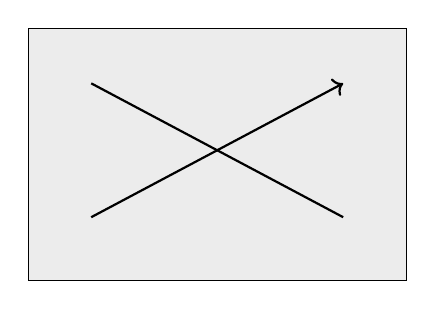
\begin{tikzpicture}
      \draw[fill=gray!15] (0,0) rectangle (4.8,3.2);
      \draw[thick,->] (0.8,0.8) -- (4,2.5);
      \draw[thick] (0.8,2.5) -- (4,0.8);
    \end{tikzpicture}
    \caption{简单示意子图}
    \label{fig:tikz-sub-left}
  \end{subfigure}
  \hfill
  \begin{subfigure}[b]{0.47\textwidth}
    \centering
    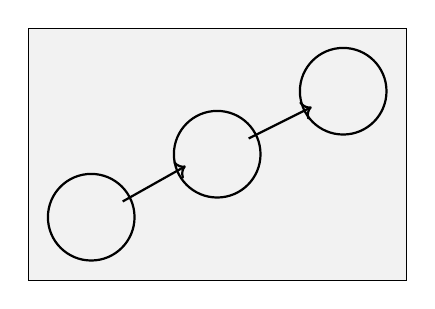
\begin{tikzpicture}
      \draw[fill=gray!10] (0,0) rectangle (4.8,3.2);
      \draw[thick] (0.8,0.8) circle [radius=0.55];
      \draw[thick] (2.4,1.6) circle [radius=0.55];
      \draw[thick] (4.0,2.4) circle [radius=0.55];
      \draw[thick,->] (1.2,1.0) -- (2.0,1.45);
      \draw[thick,->] (2.8,1.8) -- (3.6,2.2);
    \end{tikzpicture}
    \caption{并列对齐子图}
    \label{fig:tikz-sub-right}
  \end{subfigure}
  \caption{左右两个子图排版示例（TikZ）}
  \label{fig:tikz-subfigures}
\end{figure}

\cref{fig:tikz-workflow,fig:tikz-subfigures} 与上文 \texttt{graphicx} 示例的版式要求一致：图题在图下、子图可对齐引用。

\chapter{表格}\label{ch:tables}

\section{三线表示例}
\begin{table}[htbp]
  \centering
  \caption{模板常用环境与用途}
  \label{tab:booktabs}
  \begin{tabular}{lll}
    \toprule
    环境或命令 & 主要用途 & 备注 \\
    \midrule
    \texttt{\textbackslash chapter} & 一级结构组织 & 自动编号 \\
    \texttt{figure} & 插图排版 & 图题置底 \\
    \texttt{table} & 表格排版 & 表题置顶 \\
    \texttt{equation} & 单行公式 & 可交叉引用 \\
    \texttt{theorem} & 定理类内容 & 按章编号 \\
    \bottomrule
  \end{tabular}
\end{table}

\section{长表格示例}
\begin{center}
\begin{longtable}{clp{0.55\textwidth}}
  \caption{本科毕业论文（设计）组成部分说明}\\
  \toprule
  序号 & 组成部分 & 说明 \\
  \midrule
  \endfirsthead
  \caption[]{本科毕业论文（设计）组成部分说明（续）}\\
  \toprule
  序号 & 组成部分 & 说明 \\
  \midrule
  \endhead
  \bottomrule
  \endfoot
  1 & 封面 & 使用学校统一格式，体现题目、学院、专业、姓名、学号和指导教师等信息。 \\
  2 & 独创声明与授权书 & 每本论文均应附有声明页，并保留本人手写签名。 \\
  3 & 目录 & 一般列到二级标题，目录页码单独编排。 \\
  4 & 中英文摘要 & 中文在前，英文在后，需含标题、作者、单位、摘要与关键词。 \\
  5 & 导论或引言 & 交代问题背景、研究意义、研究目的和研究现状。 \\
  6 & 正文 & 论文核心部分，可根据研究内容划分多个章节。 \\
  7 & 结论 & 应准确、完整、精练，不应只是正文小结的重复。 \\
  8 & 参考文献 & 应选取查阅过且具有参考价值的权威文献，数量与外文比例须满足学校要求。 \\
  9 & 致谢 & 仅限于对论文完成有较大帮助的单位和个人。 \\
  10 & 附录 & 用于放置补充性的图表、程序、问卷或原始数据，非必须部分。 \\
\end{longtable}
\end{center}

\chapter{数学公式}\label{ch:math}

\section{编号与对齐}
模板已按章对公式编号，且可直接使用 \texttt{\textbackslash label} 与%
\texttt{\textbackslash cref} 进行交叉引用。%
例如，线性回归的最小二乘目标函数可写为
\begin{equation}
  J(\boldsymbol{\beta})=\lVert \mathbf{y}-\mathbf{X}\boldsymbol{\beta} \rVert_2^2.
  \label{eq:objective}
\end{equation}
对参数求导并令其为零，可得正规方程
\begin{align}
  \frac{\partial J}{\partial \boldsymbol{\beta}}
  &= -2\mathbf{X}^{\mathsf T}\left(\mathbf{y}-\mathbf{X}\boldsymbol{\beta}\right)=0,%
  \label{eq:gradient}\\
  \mathbf{X}^{\mathsf T}\mathbf{X}\boldsymbol{\beta}
  &= \mathbf{X}^{\mathsf T}\mathbf{y}. \label{eq:normal}
\end{align}
由 \cref{eq:objective,eq:gradient,eq:normal} 可见，单公式和对齐公式都能正确编号和引用。

考虑方程组
\begin{equation}\label{eq:uniform}
\begin{aligned}
  a\cos\theta+b\sin\theta&=10,\\
  b\cos\theta+a\sin\theta&=10
\end{aligned}
  \implies a^2+b^2=100.
\end{equation}
\eqref{eq:uniform}实现了统一编号。
\section{常见数学符号排版}
下列公式展示了常见的集合、极限、求和、积分和矩阵写法：
\begin{equation}
  A=\left\{x\in\mathbb{R}: x^2\le 1\right\}, \qquad
  \lim_{n\to\infty}\sum_{k=1}^{n}\frac{1}{k^2}=\frac{\pi^2}{6}.
\end{equation}
\begin{equation}
  \int_{0}^{1} x^\alpha (1-x)^\beta\,\mathrm{d}x
  = \frac{\Gamma(\alpha+1)\Gamma(\beta+1)}{\Gamma(\alpha+\beta+2)}.
\end{equation}
\begin{equation}
  \mathbf{A}=
  \begin{bmatrix}
    1 & 0 & 2 \\
    0 & 1 & 3 \\
    2 & 3 & 5
  \end{bmatrix}.
\end{equation}

\section{分段函数与方程组}
分段函数可用 \texttt{cases} 环境排版；例如
\[
  f(\theta):=
  \begin{cases}
    a\cos\theta,&\theta\in[\pi,2\pi),\\
    b\sin\theta,&\theta\in[0,\pi).
  \end{cases}
\]
\chapter{定理环境}\label{ch:theorem}

\section{定理、定义与证明}
\begin{defn}\label{def:convex}
若对任意 $x,y\in \mathbb{R}^n$ 和任意 $\lambda\in[0,1]$，都有
\[
f(\lambda x+(1-\lambda)y)\le \lambda f(x)+(1-\lambda)f(y),
\]
则称函数 $f$ 为凸函数。
\end{defn}

\begin{thm}[Jensen不等式]\label{thm:jensen}
设 $f$ 是定义在区间 $I$ 上的凸函数，$x_1,\dots,x_n\in I$，
$\lambda_1,\dots,$ $\lambda_n\ge 0$ 且 $\sum_{i=1}^{n}\lambda_i=1$，
则有
\[
f\!\left(\sum_{i=1}^{n}\lambda_i x_i\right)\le \sum_{i=1}^{n}\lambda_i f(x_i).
\]
\end{thm}

\begin{proof}
这是 Jensen 不等式的标准表述。对于离散情形，可由凸函数定义反复应用归纳得到。
\end{proof}

\begin{cor}\label{cor:amgm}
对任意正数 $a_1,\dots,a_n$，有
\[
\frac{a_1+\cdots+a_n}{n}\ge \sqrt[n]{a_1\cdots a_n}.
\]
\end{cor}

\begin{rmk}
在模板中，\texttt{thm}、\texttt{defn}、\texttt{cor} 等缩写环境与全称%
（\texttt{theorem}、\texttt{definition}、\texttt{corollary} 等）共享计数器，按章编号，%
并可通过 \texttt{\textbackslash cref} 直接引用，%
如 \cref{def:convex,thm:jensen,cor:amgm}。%
\end{rmk}

\chapter{参考文献引用示例}\label{ch:bib}

\noindent 本示例的 \texttt{swuthesis-main.bib} 由主文件内 \texttt{filecontents*} 环境生成；%
条目著录与公开书目一致，%
类型涵盖 GB/T~国标、西文专著、\texttt{CTeX} 手册、中文专著与期刊（可在 CNKI 等检索）、%
MathSciNet 著录的数学期刊论文、arXiv 预印本与 NeurIPS 会议论文等；%
键名与 \texttt{references.bib} 中部分条目对齐，便于对照维护。

\section{正文中的引用}
学术写作中，正文引用应与文后参考文献表一致。使用 \texttt{biblatex} 配合
GB/T 7714 样式后，可在正文中混合著录西文专著%
\cite{knuth1984texbook,lamport1994latex,mittelbach2004companion}、%
中文专著（如可在 CNKI 检索的教材）\cite{zhouzhihua2016ml}、%
中文期刊论文\cite{liguojie2012bigdata}、%
英文数学期刊（可在 MathSciNet 按 MR 号或 DOI 核对）\cite{WalpuskiZhang2021DMJ}、%
arXiv 预印本\cite{taubes2020compactness}、会议论文\cite{vaswani2017attention}；%
排版工具说明见 \cite{ctex2022}，著录格式见国家标准 \cite{gbt7714}。

\section{文后文献表}
模板默认提供参考文献章节标题，并将文献表自动加入目录。若继续扩展模板，可在这一层统一控制
文献标题、著录格式以及是否启用 \hologo{biber} 后端。

\backmatter
\printbibliography[heading=bibintoc,title={参考文献}]

\begin{ack}
行文至此，落笔为终。四载求学，倏忽而逝。回首往昔，感慨系之矣。

首谢吾师。先生治学严谨，诲人不倦。自选题立意，至谋篇布局，皆蒙悉心指点。每遇疑难，必引经据典，条分缕析，使吾豁然开朗。师恩如山，没齿难忘。今虽学业初成，然深知学海无涯，唯愿日后勤勉，不负师望。

次谢椿萱。父母劬劳，恩深似海。二十余载养育之恩，非言语所能尽述。求学之资，皆出双亲血汗；立身之道，悉承庭训熏陶。寸草春晖，难报万一。唯愿双亲康宁，以慰吾心。

亦谢同窗诸友。四载同窗，情同手足。或切磋学问，共研典籍；或漫步校园，畅叙幽情。风雨同舟，甘苦与共。今将别离，不胜依依。愿诸君前程似锦，他日重逢，情谊愈笃。

本示例文档用于展示西南大学本科毕业论文模板的主要排版功能。从封面到正文，从图表到参考文献，皆依规范而制。虽为示例，亦力求格式严谨，以资参考。

学力所限，疏漏难免。恳请师长斧正，不胜感激。

谨以此文，致谢所有关怀相助之人。

\vspace{\baselineskip}
\begin{flushright}
\begin{tabular}{c}
张三\\
\today\\
于西南大学\textbullet 李园宿舍
\end{tabular}
\end{flushright}
\end{ack}

\appendix
\chapter{西南大学本科毕业论文（设计）规范}\label{app:swu-undergrad-spec}

\noindent 为统一本科毕业论文（设计）的撰写和编辑格式，保证本科毕业论文（设计）的质量，便利信息系统的收集加工、检索利用和交流传播，在《西南大学全日制本科学生毕业论文（设计）工作管理办法》（西校〔2021〕4号）基础上，特制定本规范。

\section*{一、基本要求}
\begin{enumerate}
  \item 本科毕业论文（设计）应在导师指导下，由学生本人独立完成，严禁抄袭和剽窃。
  \item 本科毕业论文（设计）应能表明学生确已在本专业学习上掌握了专门知识，并对所研究问题有新的认识或理解，在导师的指导下具备独立解决问题的能力。论文工作时间一般不得少于半年。
  \item 原则上人文社科类专业毕业论文的字数不少于8000字，理工农医类专业毕业论文不少于6000字，%
  艺体类专业毕业论文不少于5000字；毕业论文一般应采用简体中文进行%
  （外语专业、古汉语研究中涉及的古文字和参考文献中引用的外文文献除外）；%
  如学生申请用外语进行书写，需提交申请书，由指导教师同意、系主任和学院（部）主管教学领导审批，%
  且不少于5000个单词；艺术类毕业设计说明书不少于3000字；%
  计算机软件类设计或论文，一般源程序行数不少于2000条，并写出5000字以上的软件说明书或论文。%
  各专业可根据自身特点，在学校基础上提出本专业毕业论文的具体工作量要求。
  \item 凡是不符合上述要求的，一律不接受其毕业论文（设计）答辩申请。
\end{enumerate}

\section*{二、编写格式}
\begin{enumerate}
\item 内容排列编号

毕业论文（设计）内容的顺序编号参照国家标准 GB ``标准章、条、款、项的划分编号和排列格式'' 的有关规定，采用阿拉伯数字分级编号，如：第1章第2条第2款应标为：1.2.2。

\item 论文结构（组成部分与排列顺序）

毕业论文（设计）主要由封面、独创声明与版权使用授权书、目录、中英文作者信息和摘要、导论、正文、结论、参考文献、致谢、附录等部分组成，并按此前后顺序排列。

\begin{enumerate}[label=(\arabic*)]
  \item 封面

  本科毕业论文（设计）采用白色封面。封面格式见附件1。
  \item 独创声明与版权使用授权书

  签署《毕业论文（设计）独创性声明和版权使用授权书》，其格式和内容见附件2。要求每本论文必不可缺，并有亲笔手写体签名。
  \item 目录

  目录包括论文的篇、章、条、款、项、附录等的序号、名称和页码，一般只列到二级标题。目录中文字体采用宋体小四号字，目录中的页码采用Times New Roman，小四号，1.5倍行距。目录本身的页码另编，页码在页下方居中排列，使用罗马数字（I、II……），编写格式见附件3。
  \item 中英文标题、作者信息、摘要和关键词

  另页置于目录之后，中文排在英文之前，格式见附件4，具体包含以下内容：中文标题、中文作者姓名和单位、中文内容摘要及关键词（中文摘要在300字以内，关键词3--5个）；英文标题、英文作者姓名和单位、英文摘要及关键词（英文摘要以250个实词左右为宜，关键词与中文关键词对应）。
  \item 导论（或引言）

  导论（或引言）可包括问题提出的背景、研究意义、研究目的、研究现状、研究设想、预期结果等。
  \item 正文

  正文是论文的核心部分，可根据内容分成多个章节。由于研究工作涉及的学科领域、研究方法、结果表达方式等有很大的差异，因此，对各学院（部）正文内容的撰写格式不作严格的统一要求，但每个学院内部应保持统一格式。
  \item 结论

  结论是最终的、总体的结论，不是正文中各段的小节的简单重复。结论应该准确、完整、精练。如果不可能导出应有的结论，也可以没有结论而进行必要的讨论。
  \item 参考文献

  参考文献应是论文作者查阅过的对论文具有参考价值的权威性的最新文献。参考文献的列表顺序，采用``著者-出版年制''，中外文文献分开，中文按著者姓氏拼音顺序列出、英文按字母顺序列出，中文排在前，外文排在后，连续编码，并将序号置于方括号中。所有参考文献列于正文末尾，不在各章节后列参考文献。参考文献总数应不少于10篇，其中外文资料至少2篇。
  \item 致谢

  致谢对象限于对完成毕业论文（设计）有较大帮助的单位和个人。
  \item 附录

  附录是作为论文主体的补充项目，如为了论文材料的完整性而补充的一些附加图、表等信息，并不是必须的。
\end{enumerate}
\end{enumerate}
\section*{三、排版要求}
\begin{enumerate}
\item 论文开本及版芯

论文开本大小：210\,mm$\times$297\,mm（A4纸），单面打印。版芯要求：左边距：25\,mm，右边距：25\,mm，上边距：30\,mm，下边距：25\,mm，装订线：10\,mm，页眉边距：23\,mm，页脚边距：18\,mm。

\item 标题：论文分三级标题

一级标题：黑体，四号，居中，段前、段后间距为0.5行；二级标题：黑体，小四号，段前、段后间距为0.5行；三级标题：宋体，小四号，加粗，段前、段后间距为0.5行。

\item 正文字体

正文采用小四号宋体，行间距为1.5倍；正文中的图表应有中英文对照标题，图表编号使用阿拉伯数字分章节排序。图头在图的下方，表头在表格上方，其中中文使用宋体、五号，英文及数字使用Times New Roman、五号。表格采用三线表。

论文中公式使用公式编辑器编写，格式为公式居中，编号右对齐。编号为Times New Roman、小四号。编号使用阿拉伯数字分章节排序。论文中所引用的参考文献需按在正文中出现的顺序以上标进行标注，格式为宋体、小四。

\item 页眉、页脚

除页码之外，不再设其他页眉页脚，页码采用阿拉伯数字形式，居中。

\item 量和单位

严格执行GB3100$\sim$3102：93有关量和单位的规定（参阅《常用量和单位》，计量出版社，1996）。单位名称的书写，可采用国际通用符号，也可用中文名称，但全文应统一。

\item 英文、罗马字符

英文、罗马字符一般采用Times New Roman正体，按规定应采用斜体的采用斜体。
\end{enumerate}
\section*{四、学位论文装袋顺序}
鉴于学生数量较多，由各学院（部）自行决定本单位论文是否统一打印。

装袋顺序：开题报告——教师指导学生毕业论文情况登记表——查重检测报告——指导教师评阅表——交叉评阅表——答辩记录——论文全文——图纸、作品等。

\chapter{Matlab 代码}\label{app:code-matlab}
\zihao{-4}
下面给出一个~Matlab 代码示例。该代码对应
1989年第30届国际数学奥林匹克（IMO）竞赛的一道试题的一种构造思路：\vspace{.5cm}

\noindent 求证：集合$\{1, 2, \ldots, 1989\}$可以分为$117$个互不相交的子集
\[A_i, \qquad i = 1, 2, \ldots, 117\]
使得
\begin{enumerate}[label=\arabic*., leftmargin=2em]
    \item 每个$A_i$都含有$17$个元素；
    \item 每个$A_i$中所有元素之和相同。
\end{enumerate}

代码文件名为~\path{equalsumpartition.m}，运行时在~Matlab 命令窗口输入
\begin{verbatim}
        equalsumpartition(1989,117)
\end{verbatim}
后回车即可。引入代码可使用
\begin{verbatim}
       \lstinputlisting[language=Matlab]{codes/equalsumpartition.m}
\end{verbatim}
注意：文件放在子文件夹~\path{codes/} 时，路径需写为~\path{codes/...}。

\lstinputlisting[language=Matlab]{codes/equalsumpartition.m}

\chapter{Wolfram 语言代码示例}\label{app:code-wolfram}
\begingroup
\hfuzz=1pt\relax
Wolfram 语言（Wolfram Language）为 Mathematica 所采用的标准名称；%
\texttt{listings} 宏包仍以%
\texttt{language=Mathematica}%
作为语法高亮标识，并非笔误。
\par\endgroup
按当前宏包组合，直接按第~\ref{sec:code-inclusion}~节方式引入 \path{.wl} 或笔记本导出代码时，环境配置可能仍需微调。
一种可行做法是将代码另存为 \path{.txt}，再使用
\begin{verbatim}
        \lstinputlisting[language=Mathematica]{myfile.txt}
\end{verbatim}
下面示例文件为~\path{primeSieve.txt}（与旧模板中示例同源），引入命令为
\begin{verbatim}
       \lstinputlisting[language=Mathematica]{codes/primeSieve.txt}
\end{verbatim}
该代码实现 Eratosthenes 筛法：对给定正整数$n$，可求出所有不超过$n$的素数。
示例在$[50,200]$内随机选取$n$（可修改代码中的变量 \texttt{m}、\texttt{M}）；若需查看中间过程，将变量 \texttt{d} 设为非$0$ 即可。
\lstinputlisting[language=Mathematica]{codes/primeSieve.txt}

\chapter{Python 代码}\label{app:code-python}
下面示例与 Wolfram 小节引入方式相同，文件名为~\path{test.txt}（内容对应简单的 \path{test.py} 示例）。
\begin{verbatim}
\lstinputlisting[language=Python]{codes/test.txt}
\end{verbatim}
\lstinputlisting[language=Python]{codes/test.txt}

\chapter{R 代码}\label{app:code-r}
以下示例为寿险精算中分期偿还利息与本金划分的简单演示（与旧模板示例同源），文件名为~\path{example.R}，在 \textbf{R} 中打开运行即可。
\begin{verbatim}
       \lstinputlisting[language=R]{codes/example.R}
\end{verbatim}
\lstinputlisting[language=R]{codes/example.R}

\chapter{DES 的 C++ 代码}\label{app:code-cpp}
下面示例文件为~\path{mytestdes.cpp}，实现对称密码算法~DES。
\begin{verbatim}
       \lstinputlisting[language={[ANSI]C++}]{codes/mytestdes.cpp}
\end{verbatim}
\lstinputlisting[language={[ANSI]C++}]{codes/mytestdes.cpp}

\chapter*{附录示例来源说明}
\phantomsection\label{app:source-note}
下列程序附录的例题与源码文件改编自包小敏老师长期维护的%
西南大学本科毕业论文%
\LaTeX{}模板\cite{bao2024swuthesisLegacy}（坊间常称「本科毕业论文模板\_新」等），%
原模板面向数学与统计学院本科毕业论文，版心尺寸按学校要求设置；%
其首版可追溯至 2006 年，经多年修订，近年已随学校格式调整与 \hologo{XeLaTeX} 编译方式更新。

本仓库 \texttt{swuthesis} 并非在该模板源码上直接修改，%
而是全新类文件与主文档结构；%
此处仅保留经典代码示例，便于对照 \texttt{listings} 用法。
首次使用请先阅读\cref{ch:guide}；%
公式环境见\cref{ch:math}，定理类环境见\cref{ch:theorem}；%
插图与表格分别见\cref{ch:figures}、\cref{ch:tables}；参考文献著录示例见\cref{ch:bib}；%
程序代码引入方式见\cref{sec:code-inclusion}，各语言完整示例见附录%
\ref{app:code-matlab}--\ref{app:code-cpp}。

\end{document}

\endinput
%%
%% End of file `swuthesis-main.tex'.
